\section{CFPQ Full-Stack Support}

In order to provide full-stack support of CFPQ it is necessatry to choose an appropriate graph database.
It was shown by Arseniy Terekhov et al. in~\cite{10.1145/3398682.3399163} that matrix-based algorithm can be naturally integrated into RedisGraph graph database because both, the algorithm and the database, operates over matrix representation of graphs.
Moreover, RedisGraph supports Cypher as a query language and there is a proposal which describes Cypher extension which allows one to specify context-free constraints.
Thus we choose RedisGraph as a base for our solution.  


\subsection{Cypher Extending}
\label{subsec:cypher-extension}

The first what we should do is to extend Cypher parser to be able to express context-free constraints.
There is a description of the respective Cypher syntax extension\footnote{\label{cypher-proposal}Formal syntax specification: \url{https://github.com/thobe/openCypher/blob/rpq/cip/1.accepted/CIP2017-02-06-Path-Patterns.adoc\#11-syntax}. Access date: 19.07.2020.}, proposed by Tobias Lindaaker, but this syntax does not implement yet in Cypher parsers.

This extension introduces path patterns, which are powerful alternative to the original Cypher relationship patterns.
Path patterns allow one to express regular constrains over basic patterns such as relationship and node patterns.
Like relationship patterns, they can be specified in the \texttt{MATCH} clause.

Main feature which allows one to specify context-free constraints is a \textit{named path patterns}: one can specify a name for path pattern and after that use this name in other patterns, or in the same pattern.
Named patterns can be defined in the \texttt{PATH PATTERN} clause.
Using this feature, structure of query is pretty similar to context-free grammar in the Extended Backus-Naur Form (EBNF)~\cite{EBNF_ISO}.

\begin{algorithm}
\floatname{algorithm}{Listing}
\begin{algorithmic}[1]
\caption{Query based on example grammar $G_1$ (eq.~\ref{eqn:g1_example}) in Cypher with path patterns}
\label{lst:cypher_example}
\State PATH PATTERN S = ()-/ [:c $\sim$S :d] | [:c (:y) :d] /->()
\State MATCH (v:x)-[:a | :c]->()-/ :b $\sim$S /->(to)
\State RETURN v, to
\end{algorithmic}
\end{algorithm}


The example of query which uses named path patters is presented in listing~\ref{lst:cypher_example}. 
This query is based on context-free grammar $G_1$ (eq.~\ref{eqn:g1_example}). 
Namely, path patter with name \texttt{S} specifies exactly the same constraint that specified by the grammar $G_1$. 
The \texttt{MATCH} clause uses pattern \texttt{S} in complex constraint which says that path of interest should starts in the vertex with label \texttt{x}, than in should goes throw edge with label \texttt{a} or \texttt{c}, and the end of path is a sequence of edges which starts from \texttt{b} and tail of this sequence matches with \texttt{S}.  

For the example graph $D_1$ this query returns the next pairs of vertices \texttt{(v, to)} (as specified in \texttt{RETURN} clause): !!!!

Thus this Cypher extension allows one express more complex queries including context-free path queries.
RedisGraph database supports subset of Cypher language and uses \texttt{libcypher-parser}\footnote{The \texttt{libcypher-parser} is an open-source parser library for Cypher query language. GitHub repository of the project: \url{https://github.com/cleishm/libcypher-parser}. Access date: 19.07.2020.} library to parse queries.
We extend this library by introducing new syntax proposed.
Note that we implement\footnote{The modified libsypher-pareser library with support of syntax for path patterns: \url{https://github.com/YaccConstructor/libcypher-parser}. Access date: 19.07.2020.} full extension, not only part which is necessary for simple CFPQ. 

\subsection{RedisGraph Extending}

This section describes the implementation of support for executing queries with the extended syntax in the RedisGraph. Throughout this section, we consider executing the example query from listing~\autoref{lst:cypher-example-3} for the graph $D_1$ from~\autoref{fig:example_input_graph}. $\mathcal{E}$ and $\mathcal{V}$ denotes boolean decompositions of adjacency and vertex label matrices of $D_1$ respectively. 

In the RedisGraph the main part of processing a query is building its execution plan. Execution plan consists of operations that perform basic processing such as filtering, pattern matching, aggregation and result construction. The diagram of its construction is shown in~\autoref{fig:execution-plan-construction}

After obtaining algebraic expressions they are used to construct execution plan operations. Each operation is derived from a single algebraic expression that is involved in the further execution of the corresponding operation.  During the query execution this operation performs path pattern matching and solves context-free path reachability problem if necessary. This completes the part of the query execution plan building which concerns unnamed path patterns.


The remaining part of query processing is evaluation its execution plan.

Let`s first consider the structure of the execution plan operations. Operations have parent-child relationships, so they are formed into a tree. For example, the part of execution plan that derived from example query is shown in~\autoref{fig:execution-plan-operations}. Each operation can consume a record from a child operation, process it and produce another one for the parent. Records contain information necessary for the parent operation, as well as everything to restore the response, such as identifiers of accumulated vertices and edges.


\subsection{Evaluation}

In order to demonstrate applicability of the provided extension for RedisGraph we evaluate the proposed solution on the subset of cases provided in the section~\ref{sect:py_algo_evaluation}.

For RedisGraph evaluation, we used a PC with Ubuntu 18.04 installed.
It has Intel Core i7-6700 CPU, 3.4GHz, and DDR4 64Gb RAM. 
RedisGraph with our extensions is installed form our GitHub repository\footnote{Sources of RedisGraph database with full-stack CFPQ support:\url{https://github.com/YaccConstructor/RedisGraph/tree/path_patterns_dev}. Access data: 19.07.2020.}. 

\subsubsection{Data preparing}

We use the same graphs which are presented in table~\ref{tbl:graphs_for_cfpq} to evaluate RedisGraph-based solution.

Graphs are loaded into RedisGraph database such that each vertex has a field \verb|id| which value is unique and is in $[0 \ldots |V|-1]$, where $|V|$ is a number of vertices in the graph to load.
This allows us to generate queries for specific chunk size using templates.
The template for the $g_1$ query is provided in listing~\ref{lst:query_pattern_g1}.
Here \texttt{\{id\_from\}} and \texttt{\{id\_to\}} are placeholders for lower and upper bounds for \verb|id|. The example of the exact query for chunk of size 16 is presented in listing~\ref{lst:query_g1}.

\begin{algorithm}
\floatname{algorithm}{Listing}
\begin{algorithmic}[1]
\caption{Cypher query pattern for $g_1$}
\label{lst:query_pattern_g1}
\State PATH PATTERN S =  \par
 \hskip\algorithmicindent ()-/ [<:SubClassOf [$\sim$S | ()] :SubClassOf] \par
 \hskip\algorithmicindent | [<:Type [$\sim$S | ()] :Type] /->()
\State MATCH (src)-/ $\sim$S /->() 
\State WHERE \{id\_from\} <= src.id and src.id <= \{id\_to\}
\State RETURN count(*)
\end{algorithmic}
\end{algorithm}

\begin{algorithm}
\floatname{algorithm}{Listing}
\begin{algorithmic}[1]
\caption{Query $g_1$ in Cypher using the template from listing~\ref{lst:query_pattern_g1}}
\label{lst:query_g1}
\State PATH PATTERN S =  \par
 \hskip\algorithmicindent ()-/ [<:SubClassOf [$\sim$S | ()] :SubClassOf] \par
 \hskip\algorithmicindent | [<:Type [$\sim$S | ()] :Type] /->()
\State MATCH (src)-/ $\sim$S /->() 
\State WHERE 15 <= src.id and src.id <= 31
\State RETURN count(*)
\end{algorithmic}
\end{algorithm}

Queries generator for all three queries ($g_1$, $g_2$, and $geo$) was implemented and used to create queries for all chunks which are used in the previous experiment. 


\subsubsection{Evaluation results}

For evaluation we select $geo$ query for \textit{geospecies} graph as one of the hardest queries, and $g_1$ query for other graphs.
Time and memory consumption are measured for each chunk processing.
Results of time measurement are presented in figures~\ref{fig:redis_core_all}--\ref{fig:redis_gohierarchy_all}.

\begin{figure}[h]
\centering
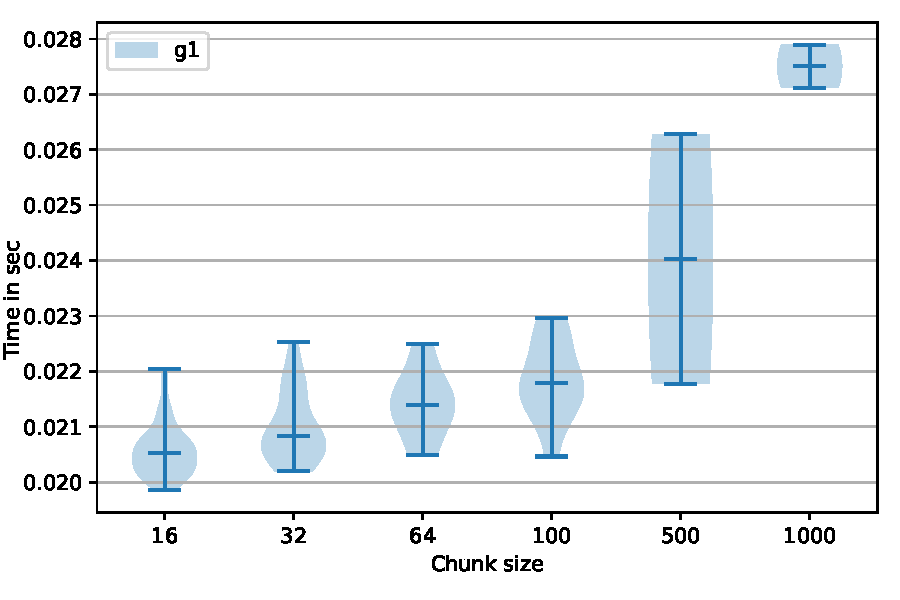
\includegraphics[width=0.45\textwidth]{data/raw_redis/core.pdf}
\caption{RedisGraph performance on \textit{core} graph}
\label{fig:redis_core_all}
\end{figure}


\begin{figure}[h]
\centering
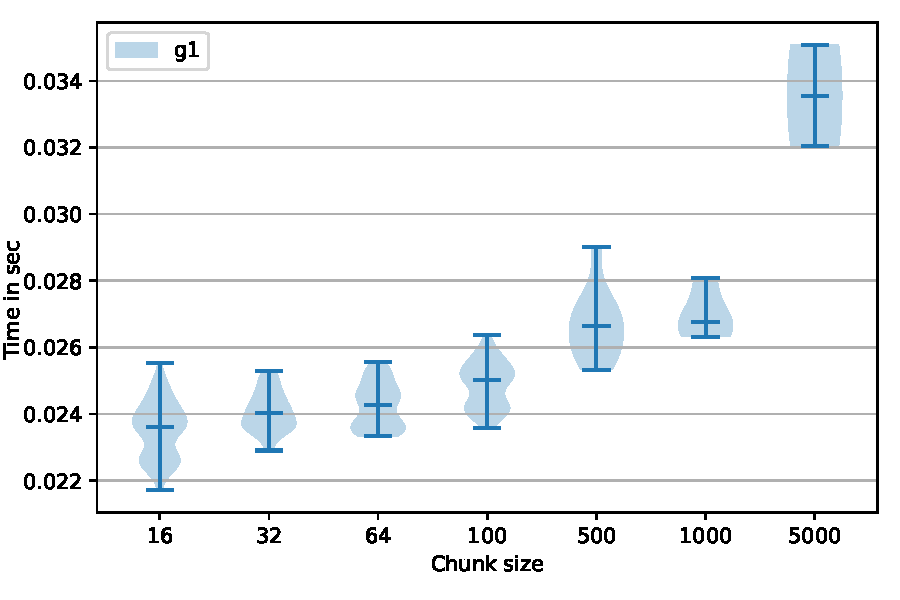
\includegraphics[width=0.45\textwidth]{data/raw_redis/pathways.pdf}
\caption{RedisGraph performance on \textit{pathways} graph}
\label{fig:redis_pathways_all}
\end{figure}

\begin{figure}[h]core
\centering
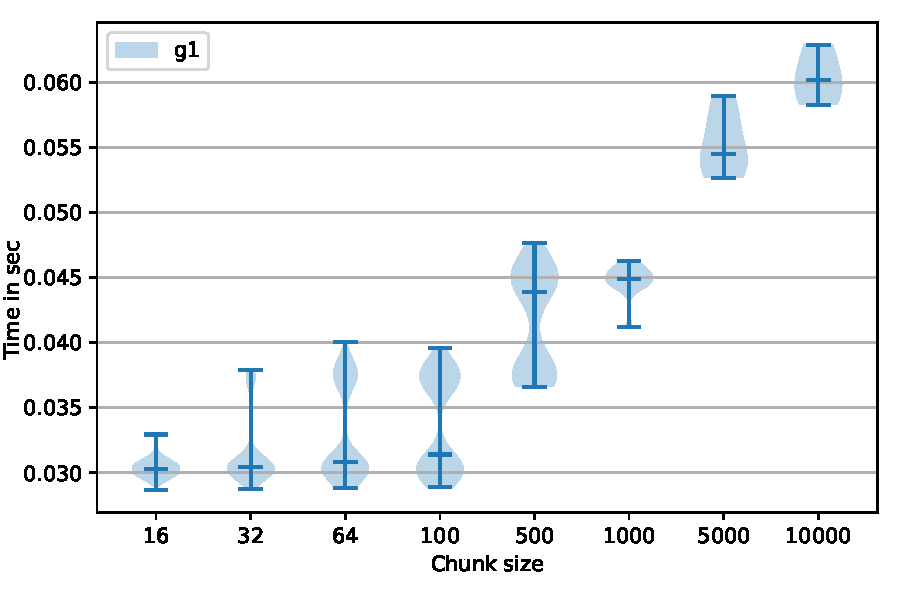
\includegraphics[width=0.45\textwidth]{data/raw_redis/enzyme.pdf}
\caption{RedisGraph performance on \textit{enzyme} graph}
\label{fig:redis_enzyme_all}
\end{figure}


\begin{figure}[h]
\centering
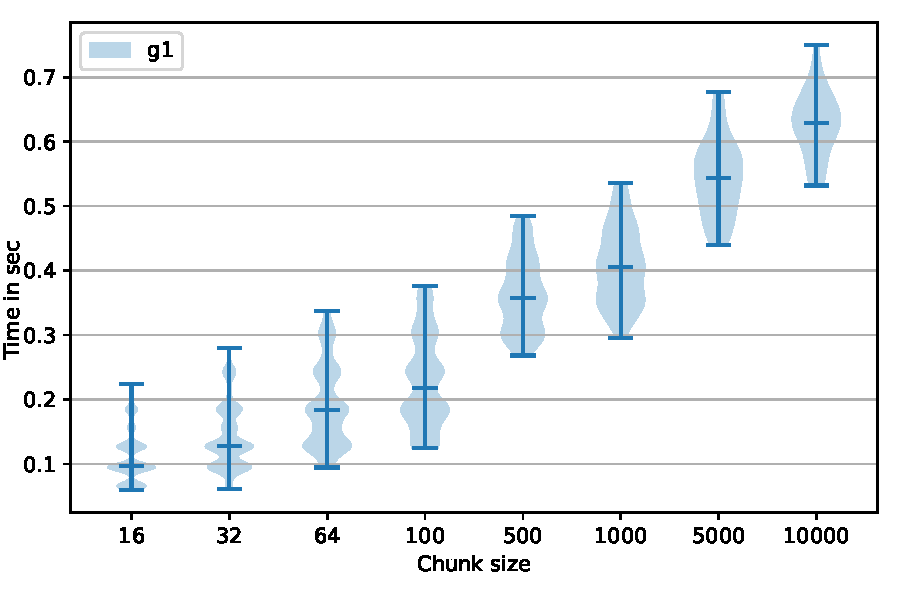
\includegraphics[width=0.45\textwidth]{data/raw_redis/go.pdf}
\caption{RedisGraph performance on \textit{go} graph}
\label{fig:redis_go_all}
\end{figure}

\begin{figure}[h]
\centering
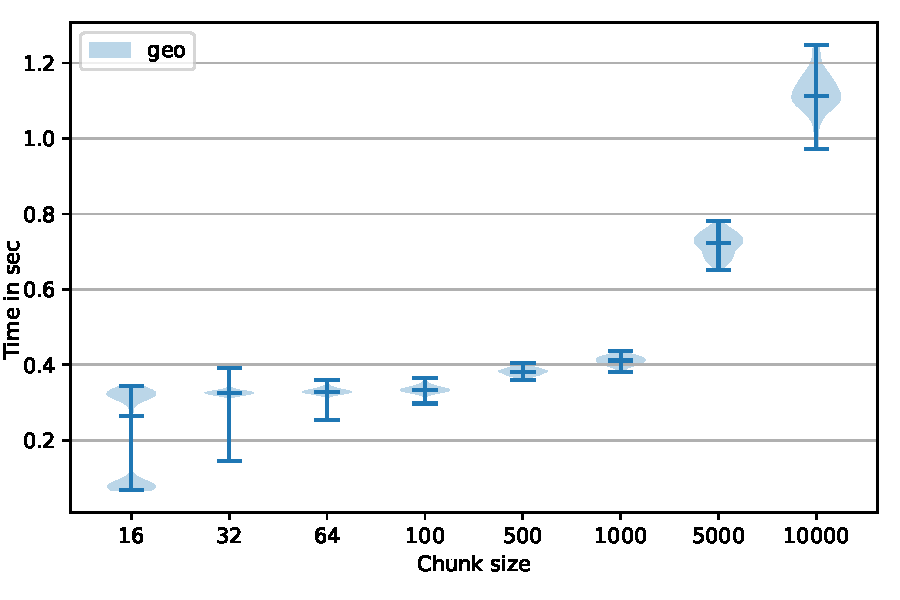
\includegraphics[width=0.45\textwidth]{data/raw_redis/geospecies.pdf}
\caption{RedisGraph performance on \textit{geospecies} graph}
\label{fig:redis_geospecies_all}
\end{figure}

\begin{figure}[h]
\centering
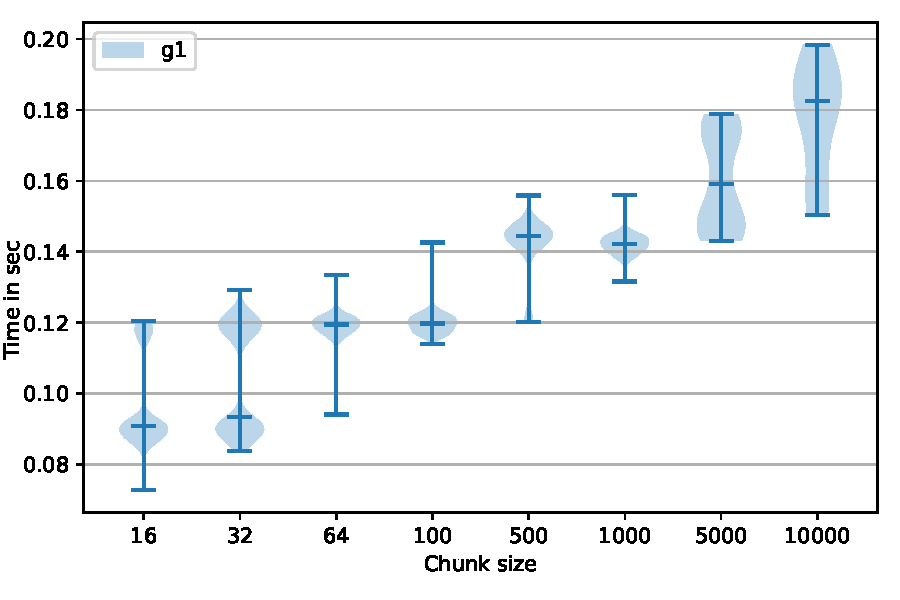
\includegraphics[width=0.45\textwidth]{data/raw_redis/eclass_514en.pdf}
\caption{RedisGraph performance on \textit{eclass\_514en} graph}
\label{fig:redis_eclass_all}
\end{figure}

\begin{figure}[h]
\centering
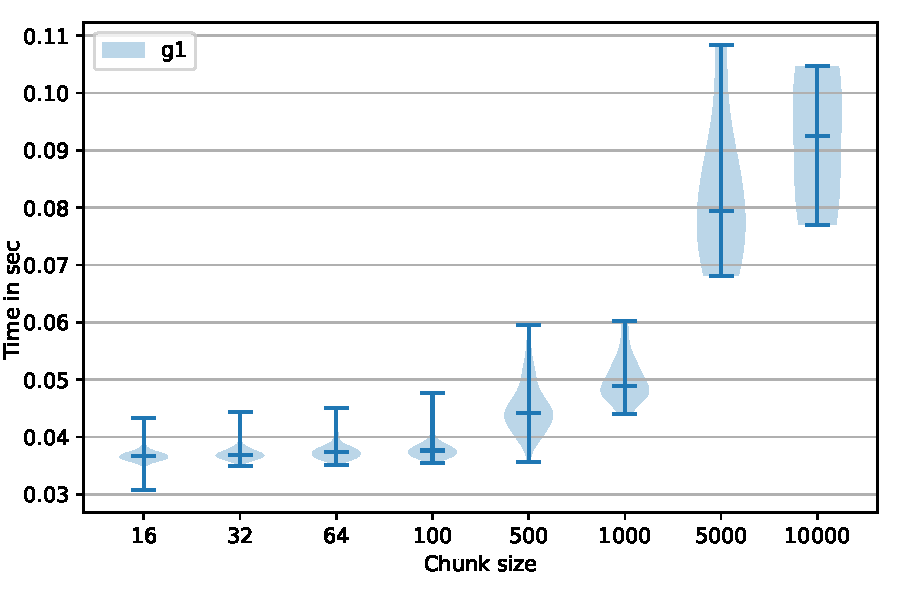
\includegraphics[width=0.45\textwidth]{data/raw_redis/gohierarchy.pdf}
\caption{RedisGraph performance on \textit{gohierarchy} graph}
\label{fig:redis_gohierarchy_all}
\end{figure}

We can see, that results is comparable with one given in section~\ref{sect:py_algo_evaluation}. 
Processing time for all chunks, except chunk of size 10~000 for \textit{geospecies} graph (fig.~\ref{fig:redis_geospecies_all}) is less then 1 second.
Moreover, for chunks of size 16 processing median time is less then 0.1 second, except \textit{geospecies} graph.

Memory consumption for two big graphs \textit{eclass\_514en} and \textit{geospecies} is presented in figures~\ref{fig:redis_memory_eclass} and~\ref{fig:redis_memory_geospecies} respectively.
We can see, that amount of used memory depends on graph and query, but for relatively small chunks ($\leq 1000$) RedisGraph uses less that 50Mb of RAM to process one chunk.
Note that RedisGraph includes memory management system, thus in our experiments all allocated memory is measured, not only really used for query evaluation.
As a result, we can conclude that multiple-source CFPQ is significantly more memory efficient than creation of full reachability index and its filtering: processing the chunk of size 10~000 on \textit{geospecies} graph requires less than 200Mb, while full index creation requires 16Gb~\cite{10.1145/3398682.3399163}.  

\begin{figure}[h]
\centering
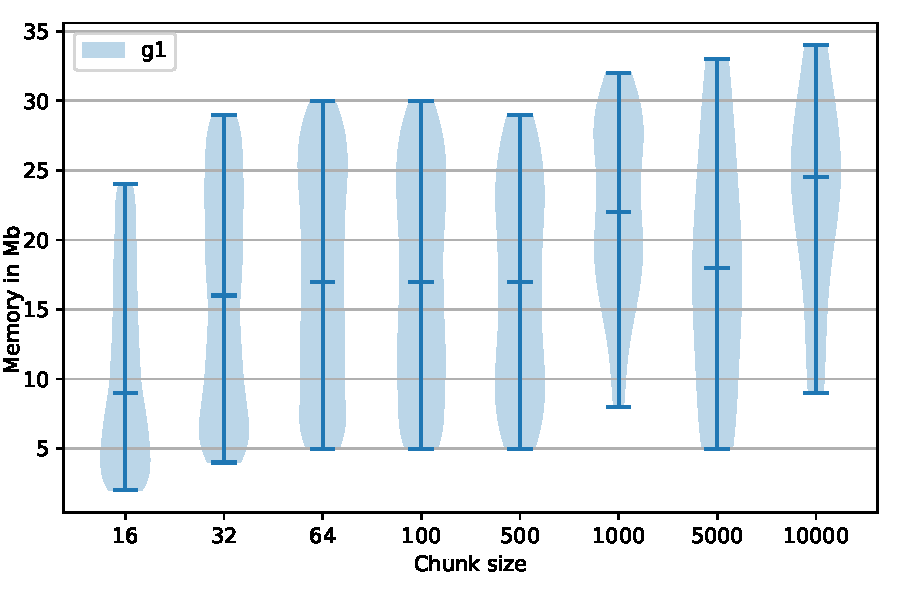
\includegraphics[width=0.5\textwidth]{data/raw_memory/eclass_514en.pdf}
\caption{RedisGraph memory consumption on \textit{eclass\_514en} graph}
\label{fig:redis_memory_eclass}
\end{figure}

\begin{figure}[h]
\centering
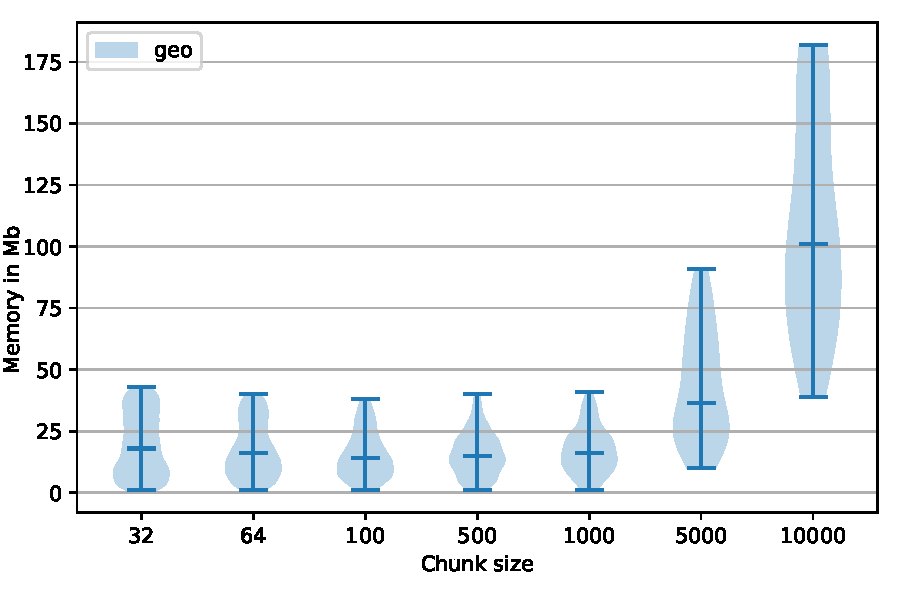
\includegraphics[width=0.5\textwidth]{data/raw_memory/geospecies.pdf}
\caption{RedisGraph memory consumption on \textit{geospecies} graph}
\label{fig:redis_memory_geospecies}
\end{figure}


Additionally, we measure the time required to process full graph (to solve all-pairs reachability problem) by chunks of size 1000.
Total processing time (in seconds) and total required memory (in Mb) are measured.
Also, we compare our solution with results of Arseniy Terekhov et al. from~\cite{10.1145/3398682.3399163} which were measured for RedisGraph deployed on the similar hardware and for the same graphs and queries.
In~\cite{10.1145/3398682.3399163} Azimov's algorithm was naively integrated with RedisGraph storage without support of query language and other mechanisms such as lazy query evaluation.
Results are provide in the table~\ref{tbl:redis_full_graph_processing}.

{\setlength{\tabcolsep}{0.25em}
\begin{table}
{
\caption{Full graph processing time by RadisGraph with chunks of size 1000, time is measured in seconds, memory in Mb (\textbf{Chunks} --- the proposed solution, \textbf{Mono} --- results from~\cite{10.1145/3398682.3399163})}
\label{tbl:redis_full_graph_processing}
\small
\rowcolors{3}{black!2}{black!10}
\begin{tabular}{|l|c|c|c|c|c|c|}
\hline
\multirow{2}{*}{Graph} & \multirow{2}{*}{\#V} & \multirow{2}{*}{\#E} & \multirow{2}{*}{Query} & \multicolumn{2}{c|}{Chunks}  &  \multirow{2}{*}{Mono}  \\
                       &                      &                      &                        & Time   & Mem & \\
\hline
\hline
core                   & 1323                 & 3636                 & $g_1$                  & 0.003  & 2                  &  0.004 \\ 
pathways               & 6238                 & 18 598               & $g_1$                  & 0.031  & 6                  &  0.011 \\ 
gohierarchy            & 45 007               & 980 218              & $g_1$                  & 0.847  & 62                  &  0.091 \\ 
enzyme                 & 48 815               & 117 851              & $g_1$                  & 0.698  & 13                  &  0.018 \\ 
eclass\_514en          & 239 111              & 523 727              & $g_1$                  & 18.825 & 35                   &  0.067 \\ 
geospecies             & 450 609              & 2 311 461            & $geo$                  & 80.979 & 196                  &  7.146 \\
go                     & 582 929              & 1 758 432            & $g_1$                  & 72.034 & 40                  &  0.604 \\ 
\hline
\end{tabular}
}
\end{table}
}

We can see, that chunk-by-chunk processing is slower, but it is still require reasonable time.
First of all, if chunk size is comparable with graph size (\textit{core} and \textit{pathways} graphs) then time to processing is comparable with monolithic processing.
Thus one can decrease time to process by increasing of chunk size and gets near optimal time.
On the other hand, even with relatively small chunks (\textit{eclass\_514}, \textit{go} and \textit{geospecies} graphs), when for chunk-by-chunk processing requires more than 100 times more time, our results still reasonable for some cases. 
For example, it requires more than 70 times less time for \textit{geospecies} grap processing than solution of Jochem Kuijpers et al.~\cite{Kuijpers:2019:ESC:3335783.3335791} which is based on Neo4j and requires more than 6000 seconds.
Moreover, while solution from~\cite{10.1145/3398682.3399163} requires huge amount of memory (more than 16Gb for \textit{geospecies} graph and $geo$ query), our solution requires only 196Mb in the same scenario.
Thus it is more suitable for general-purpose graph databases: main scenario---relatively small start vertices set---can be handled efficiently, and all-pairs reachability, which is not a massive case, can be solved in reasonable time with low memory consumption. In specific cases one can easy tune our solution to get optimal time and memory consumption.

Finally we can conclude that provided solution is a promising way to implement CPFQ for real-world graph databases.